\documentclass[conference]{IEEEtran}

\usepackage{graphicx}
\usepackage{booktabs}
\usepackage{url}
\usepackage{cite}
\usepackage[caption=false,font=footnotesize]{subfig}

\title{Sandbox-Based Capacity Characterization of Hotel Reservation Microservices}

\author{
\IEEEauthorblockN{Sathish and Team}
\IEEEauthorblockA{Semester 6 SSP Project\\
DeathStarBench Hotel Reservation Sandboxing Study}
}

\begin{document}
\maketitle

\begin{abstract}
We document a sandboxing and capacity-analysis workflow for the DeathStarBench Hotel Reservation application. Instead of benchmarking the system only end to end, we isolate individual microservices and estimate their Microservice Capacity (MSC), defined as the highest request rate that satisfies a success-rate and latency service-level objective (SLO). Our implementation combines two paths. First, we evaluate \texttt{search} inside a dependency sandbox built from captured gRPC traffic, where downstream \texttt{geo} and \texttt{rate} are replaced by deterministic replay services. Second, we directly stress leaf services such as \texttt{geo}, \texttt{rate}, \texttt{profile}, \texttt{recommendation}, \texttt{user}, and \texttt{reservation} under controlled CPU and replica settings. We also train per-service linear models to predict MSC for unseen configurations. Across collected runs, \texttt{search} achieved the highest observed MSC and reached the configured test ceiling of 500 RPS at 500m CPU with two replicas, while \texttt{rate} remained the weakest service overall. When we compared sandboxed and live \texttt{search} under the same SLO, the sandbox average was 151.1 RPS versus only 19.6 RPS live, showing that sandboxing removed dependency noise and exposed the capacity of \texttt{search} itself. A follow-up bottleneck investigation indicates that \texttt{rate} is limited by CPU throttling at low CPU budgets and by cold-cache fan-out and coordination overhead even after throttling disappears. Our 150m validation experiment achieved a mean absolute percentage error of 16.4\% across six services, showing that the trained model is useful for coarse capacity estimation.
\end{abstract}

\begin{IEEEkeywords}
microservices, sandboxing, capacity modeling, Kubernetes, performance analysis, DeathStarBench
\end{IEEEkeywords}

\section{Introduction}
Microservice applications are difficult to capacity-plan because each service has different compute intensity, fan-out behavior, latency sensitivity, and cache behavior. In the Hotel Reservation benchmark, a single user-facing request may traverse several gRPC services and infrastructure components. End-to-end benchmarking is therefore necessary, but it does not directly answer the service-level questions we care about: which microservice is the bottleneck, which resource change helps, and what throughput can we expect from a new deployment configuration.

We address this problem through sandbox-based measurement. We measure a service in controlled isolation while preserving realistic traffic semantics. Following the MSC idea from prior cloud microservice performance-modeling work~\cite{jindal2019}, we define Microservice Capacity as the highest request rate that still satisfies both success-rate and latency SLOs. Our work is not a reproduction of the reference paper. Instead, it is an implementation-focused project report describing the logic we built, the experiments we ran, and the insights we obtained on Hotel Reservation from DeathStarBench~\cite{gan2019}.

Our repository implements a complete workflow that captures gRPC traffic, converts it into deterministic replay fixtures, renders a dedicated Kubernetes sandbox, performs binary-search load testing, trains simple MSC prediction models, and investigates bottlenecks in depth when scaling breaks down. The main contribution of this report is practical: we show how we turned a benchmark application into a reproducible service-level capacity-analysis framework.

\section{Workflow and Sandboxing Design}
\subsection{System Context}
Within the portion of Hotel Reservation we studied, \texttt{search} depends on \texttt{geo} and \texttt{rate}. The other evaluated services, namely \texttt{geo}, \texttt{rate}, \texttt{profile}, \texttt{recommendation}, \texttt{user}, and \texttt{reservation}, can be stress-tested directly in our setup. This naturally led us to two complementary workflows:
\begin{enumerate}
\item dependency sandboxing for \texttt{search}, and
\item direct leaf-service MSC measurement.
\end{enumerate}

This separation is important. If we benchmark \texttt{search} against the live cluster, downstream variability from \texttt{geo} and \texttt{rate} contaminates the result. If we benchmark only leaf services, we miss the behavior of a dependency-heavy microservice. We therefore use both paths and combine their outputs in a single analysis dataset.

It is also the reason we applied sandboxing only to \texttt{search}. In our selected set of services, \texttt{search} is the only target whose throughput and latency are directly coupled to downstream service behavior. The other services in our study are effectively leaf services in this workflow, so direct MSC measurement is sufficient for them. In other words, sandboxing is not something we applied everywhere by default; we used it precisely where a service-level measurement would otherwise be obscured by dependency effects.

\subsection{Traffic Capture and Replay Fixtures}
We added a unary gRPC interceptor to baseline services so that, when capture mode is enabled, each request produces one NDJSON record containing timestamp, service, method, request payload, response payload, gRPC code, and duration. The capture stage is driven by warm-up traffic through the baseline application, so the recorded traces reflect real application calls rather than synthetic protocol-only examples.

We then normalize the captured traffic before turning it into sandbox fixtures. The normalization stage canonicalizes JSON payloads, rounds floating-point fields, deduplicates repeated request-response pairs, and stores fixtures indexed by method plus normalized request. This gives us deterministic replay behavior while still preserving realistic request shapes and response content.

We also handle a specific correctness corner case in the \texttt{search} pipeline. If a \texttt{geo} lookup returns no hotels, then the corresponding \texttt{rate} request should also be valid for an empty hotel set. We therefore add synthetic empty-rate fixtures derived from the captured search corpus. Without this step, \texttt{search} can fail inside the sandbox on legitimate empty-result inputs even though the live system handles them correctly.

\subsection{Search Sandboxing Procedure}
Our \texttt{search} experiment runs in six stages:
\begin{enumerate}
\item send baseline warm-up requests through the frontend,
\item capture live \texttt{search}, \texttt{geo}, and \texttt{rate} traffic,
\item build \texttt{geo} and \texttt{rate} replay fixtures plus a \texttt{search} request corpus,
\item create a fresh sandbox namespace,
\item deploy deterministic dummy \texttt{geo} and \texttt{rate} services, and
\item load-test sandboxed \texttt{search} under different CPU and replica settings.
\end{enumerate}

The dummy services register through Consul so that \texttt{search} continues to resolve downstream dependencies through the normal service-discovery path. This matters because we wanted a replay-based sandbox, not a handwritten shortcut around the application network structure.

Another subtle but important implementation detail is the way requests are distributed across \texttt{search} replicas. Once local port-forwards are established, we create one gRPC stub per forwarded pod and cycle through them in round-robin order. We also warm every replica before the measured interval begins. This avoids a biased experiment in which early traffic sticks to one pod and makes multi-replica configurations look weaker than they actually are. In other words, our replica sweeps exercise the whole \texttt{search} pool instead of accidentally measuring just one hot pod.

\subsection{Leaf-Service Experiments}
For leaf services, we bypass dependency sandboxing and issue gRPC calls directly to the service under test. Each service has a curated request corpus designed to vary the request shape. For example, \texttt{rate} uses different hotel IDs and date windows, \texttt{profile} mixes single-hotel and full-batch requests, and \texttt{user} checks many seeded Cornell user credentials.

We also intentionally control cache state. For services backed by Memcached, namely \texttt{rate}, \texttt{profile}, and \texttt{reservation}, we flush Memcached before each load step by launching a short-lived helper pod that sends \texttt{flush\_all} to the cache service. This makes each step start from a colder state and yields a more conservative MSC. The benefit is methodological consistency: capacity numbers are not inflated by warmed cache entries left behind from earlier steps in the binary search.

\subsection{MSC Measurement Logic}
We measure MSC using binary search over offered request rate. A candidate rate is accepted only when two conditions hold:
\begin{enumerate}
\item success rate is at least 0.99, and
\item P90 latency is at most 100 ms.
\end{enumerate}

The regression sweeps evaluate CPU values of 100m, 200m, and 500m, and replica counts of 1, 2, and 3. For each configuration, we store the best accepted RPS as MSC together with the observed pod CPU reported by Kubernetes metrics. This produces a dataset that is useful both for visual analysis and for later model fitting.

The request-level timeout remains fixed at 0.3 s for both sandboxed and live \texttt{search} runs. This is important for fair comparison. If the timeout or SLO were different across the two paths, then any observed MSC gap could be attributed to measurement settings rather than to the presence or absence of dependency sandboxing.

\section{Experimental Results}
\subsection{Cross-Service Comparison}
Across seven evaluated services, we observed major heterogeneity in MSC. Fig.~\ref{fig:service-comparison} compares average MSC across all tested configurations. The strongest average services are \texttt{user} at 194.44 RPS and \texttt{recommendation} at 184.44 RPS. The weakest is \texttt{rate} at 86.67 RPS. \texttt{search} still ranks strongly at 151.11 RPS even though it is measured in a dependency-aware sandbox rather than as a direct leaf service.

\begin{figure}[t]
\centering
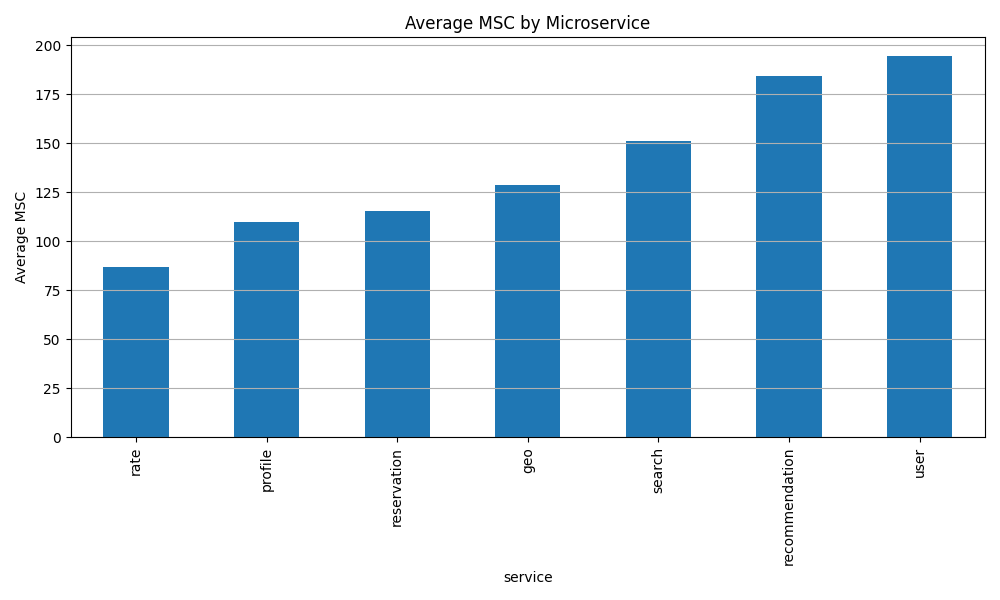
\includegraphics[width=\columnwidth]{report_figures/service_comparison_avg_msc.png}
\caption{Average MSC across evaluated microservices.}
\label{fig:service-comparison}
\end{figure}

Table~\ref{tab:best-configs} summarizes the best observed configuration for each service. Two points stand out. First, \texttt{search} reaches the configured experimental ceiling of 500 RPS at 500m CPU with two replicas, so its true saturation point may be higher. Second, the best configuration is not always the largest one. \texttt{recommendation}, for example, already reaches 320 RPS at 200m with three replicas, showing that service-level scaling behavior is not simply monotonic in CPU.

\begin{table}[t]
\caption{Best Observed Configuration per Service}
\label{tab:best-configs}
\centering
\begin{tabular}{lccc}
\toprule
Service & CPU (m) & Replicas & Best MSC \\
\midrule
Search & 500 & 2 & 500 \\
Reservation & 500 & 3 & 380 \\
Geo & 500 & 3 & 320 \\
Recommendation & 200 & 3 & 320 \\
Profile & 500 & 2 & 310 \\
User & 500 & 3 & 280 \\
Rate & 500 & 3 & 230 \\
\bottomrule
\end{tabular}
\end{table}

\subsection{Search Sandbox Behavior}
Fig.~\ref{fig:search-results} shows the main trends for the sandboxed \texttt{search} service. At 100m CPU, additional replicas do not help much; the MSC remains low and two replicas give no improvement over one. At 200m CPU, however, the jump from two to three replicas increases MSC from 50 to 145 RPS. This indicates that \texttt{search} benefits strongly from additional parallelism once enough aggregate compute is available. At 500m CPU, both the two-replica and three-replica configurations reach the 500 RPS test cap.

\begin{figure*}[t]
\centering
\subfloat[Search MSC versus CPU]{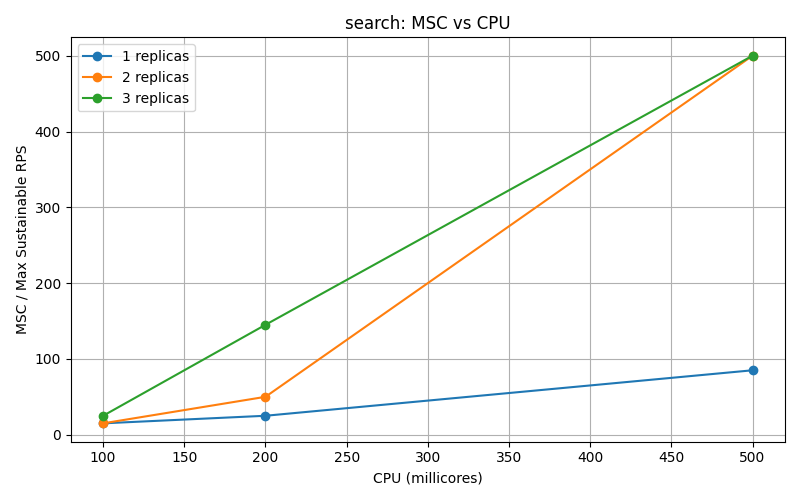
\includegraphics[width=0.48\textwidth]{report_figures/search_msc_vs_cpu.png}}
\hfill
\subfloat[Search MSC versus replicas]{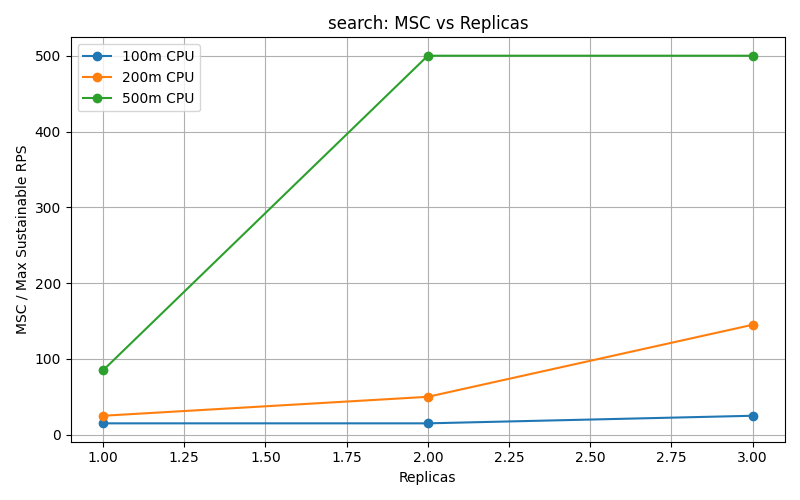
\includegraphics[width=0.48\textwidth]{report_figures/search_msc_vs_replicas.png}}
\caption{Capacity trends for sandboxed \texttt{search}.}
\label{fig:search-results}
\end{figure*}

These results validate the sandbox methodology itself. We preserved realistic request structure and downstream responses through capture-and-replay, but we removed the run-to-run noise of live downstream services. As a result, the effect of changing CPU or replica count on \texttt{search} becomes much easier to interpret.

\subsection{Live Versus Sandboxed Search}
To test whether sandboxing genuinely helped us isolate \texttt{search}, we also ran the same \texttt{search} MSC procedure directly against the live baseline system, where real \texttt{geo} and \texttt{rate} remained on the critical path. The comparison is decisive. Across the same nine CPU/replica configurations, sandboxed \texttt{search} averaged 151.1 RPS, while live \texttt{search} averaged only 19.6 RPS. The median MSC advantage of sandboxing was 30 RPS, and the largest gains appeared at the higher-resource settings where live \texttt{search} remained strongly latency-bound.

\begin{table}[t]
\caption{Sandboxed Versus Live Search MSC}
\label{tab:search-compare}
\centering
\begin{tabular}{ccccc}
\toprule
CPU (m) & Replicas & Sandbox & Live & Delta \\
\midrule
100 & 1 & 15 & 1 & +14 \\
100 & 2 & 15 & 10 & +5 \\
100 & 3 & 25 & 25 & 0 \\
200 & 1 & 25 & 15 & +10 \\
200 & 2 & 50 & 20 & +30 \\
200 & 3 & 145 & 25 & +120 \\
500 & 1 & 85 & 25 & +60 \\
500 & 2 & 500 & 30 & +470 \\
500 & 3 & 500 & 25 & +475 \\
\bottomrule
\end{tabular}
\end{table}

Table~\ref{tab:search-compare} makes the pattern clear. At 500m CPU with two replicas, sandboxed \texttt{search} reaches the experiment ceiling of 500 RPS, while live \texttt{search} reaches only 30 RPS. At 500m with three replicas, the gap is 475 RPS. Even at 200m with three replicas, the sandbox reaches 145 RPS while the live system reaches only 25 RPS.

The failure mode also matters. In the live runs, every configuration violated the P90 latency requirement rather than the success-rate requirement. This shows that the live application could often still return requests, but the response-time inflation from downstream dependency behavior prevented us from treating the result as the capacity of \texttt{search} itself. In contrast, once \texttt{geo} and \texttt{rate} were replaced with deterministic replay services, the measured MSC reflected the behavior of \texttt{search} much more directly.

This comparison gives us the strongest practical argument for sandboxing in the entire project. Without sandboxing, we would conclude that \texttt{search} is a weak service whose capacity remains below 30 RPS in most cases. With sandboxing, we see that \texttt{search} can scale to far higher throughput and that much of the live bottleneck actually comes from dependency interaction rather than from the \texttt{search} implementation alone. Sandboxing therefore did exactly what we wanted: it allowed us to measure the performance of a single microservice, here \texttt{search}, instead of repeatedly measuring the combined behavior of \texttt{search}, \texttt{geo}, and \texttt{rate}.

\subsection{Leaf-Service Scaling Trends}
Fig.~\ref{fig:reservation-rate} compares two representative leaf-service behaviors. \texttt{reservation} scales aggressively at higher CPU budgets and reaches 380 RPS at 500m with three replicas. \texttt{rate}, in contrast, scales weakly and shows poor replica efficiency. Even before the detailed bottleneck study, the aggregate plots suggest that \texttt{rate} is the most likely system bottleneck.

\begin{figure*}[t]
\centering
\subfloat[Reservation MSC versus CPU]{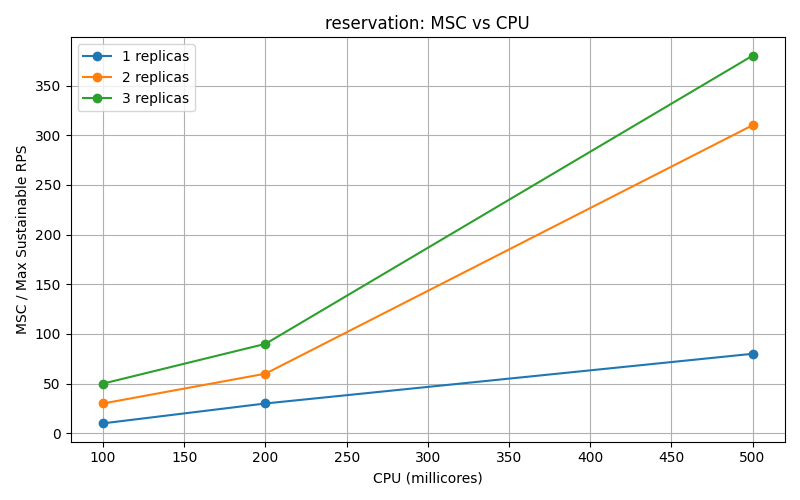
\includegraphics[width=0.32\textwidth]{report_figures/reservation_msc_vs_cpu.png}}
\hfill
\subfloat[Rate MSC versus CPU]{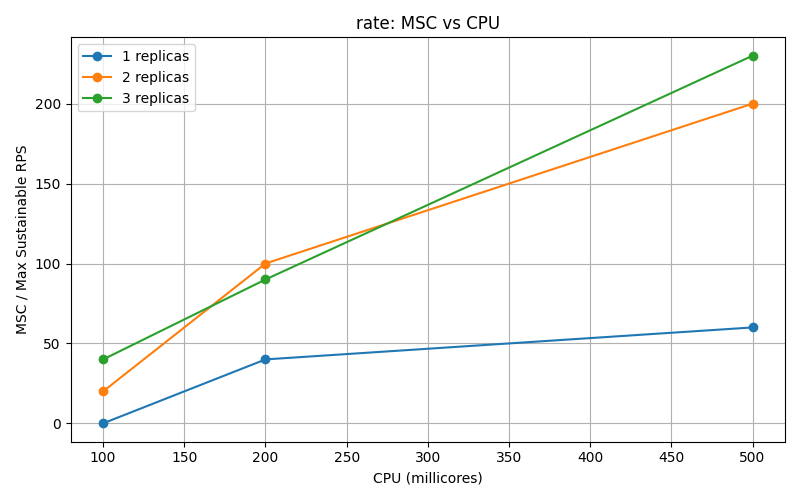
\includegraphics[width=0.32\textwidth]{report_figures/rate_msc_vs_cpu.png}}
\hfill
\subfloat[Rate replica scaling efficiency]{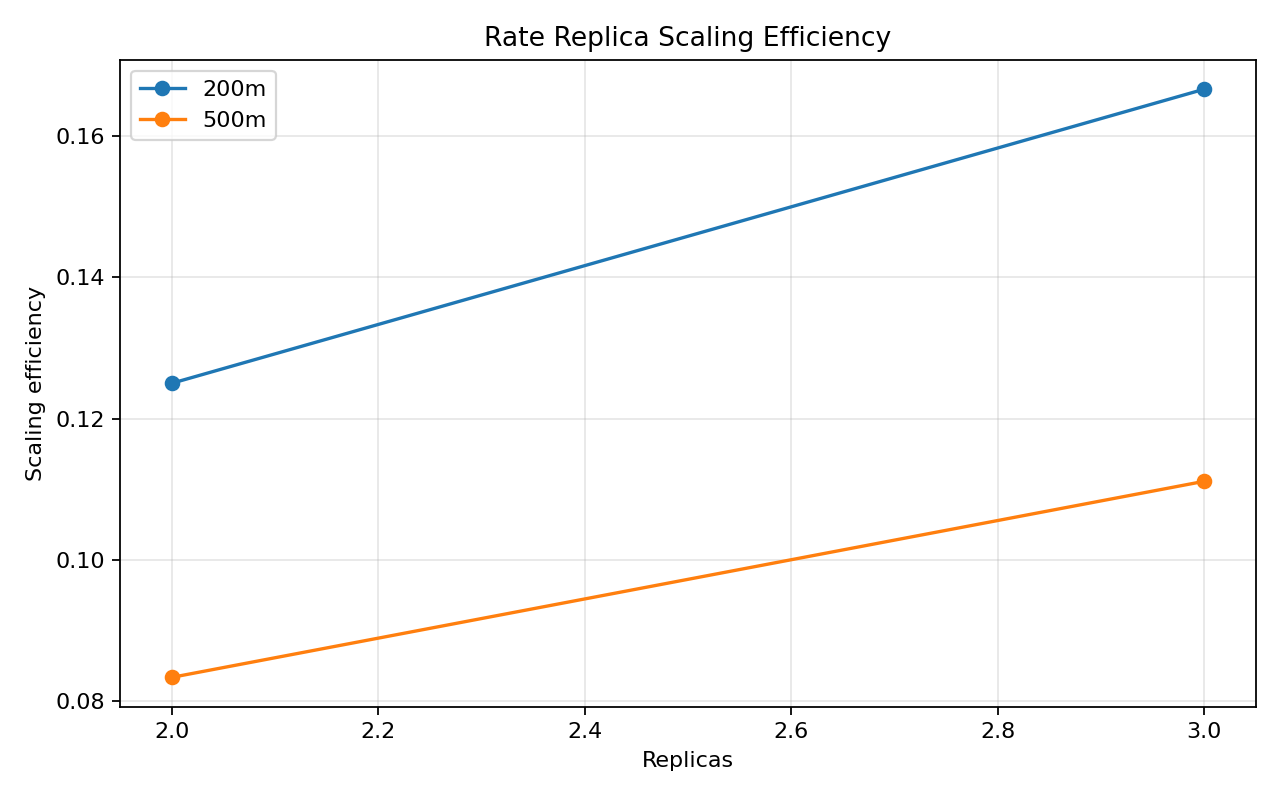
\includegraphics[width=0.32\textwidth]{report_figures/replica_scaling_efficiency.png}}
\caption{Representative scaling behavior for \texttt{reservation} and \texttt{rate}.}
\label{fig:reservation-rate}
\end{figure*}

The contrast between the two services is useful. Both are measured under the same experimental logic, but only \texttt{rate} shows persistently weak gains from extra replicas. This tells us that the bottleneck is not an artifact of the measurement harness alone. It is tied to the service's own runtime behavior.

\section{Predictive MSC Modeling}
\subsection{Per-Service Model}
After collecting the regression data, we added a lightweight prediction layer to estimate MSC for unseen configurations. Instead of fitting one global model for all services, we train one model per service. This reflects our earlier observation that scaling behavior differs substantially across services.

The current model uses only features available at deployment time:
\begin{enumerate}
\item CPU millicores per pod, and
\item replica count.
\end{enumerate}

For each service, we fit either a constant model when only one clean point is available or a linear model of the form
\[
\text{MSC} = \beta_0 + \beta_1 \cdot \text{CPU} + \beta_2 \cdot \text{Replicas}.
\]
Before fitting, we exclude rows with zero MSC and rows marked as \texttt{max\_rps\_reached}. The zero-MSC rows are treated as artifacts or degenerate cases, while the \texttt{max\_rps\_reached} rows are censored because the experiment ended before true saturation was observed.

\subsection{Validation on Unseen 150m CPU Runs}
To test whether the learned models generalize beyond the training grid, we ran a separate validation experiment at 150m CPU, a value not present in the original 100m/200m/500m sweep. Table~\ref{tab:validation} summarizes the results for the six leaf services included in the validation dataset. Across these held-out points, the mean absolute percentage error (MAPE) is 16.4\%.

\begin{table}[t]
\caption{Validation Results at 150m CPU}
\label{tab:validation}
\centering
\begin{tabular}{lccc}
\toprule
Service & Replicas & Actual MSC & Predicted MSC \\
\midrule
Geo & 2 & 70 & 74.7 \\
Rate & 2 & 40 & 42.6 \\
Profile & 2 & 40 & 53.9 \\
Recommendation & 2 & 170 & 147.9 \\
User & 2 & 200 & 160.2 \\
Reservation & 2 & 40 & 47.1 \\
\bottomrule
\end{tabular}
\end{table}

The model performs best on \texttt{geo} and \texttt{rate}, where the prediction errors are 6.8\% and 6.5\%, respectively. It performs worst on \texttt{profile}, where the error rises to 34.8\%. This pattern is reasonable: a two-feature linear model can approximate smooth scaling trends, but it cannot capture stronger non-linearities, cache effects, or saturation plateaus. Even so, a 16.4\% mean error is good enough to support coarse capacity planning and to narrow the configurations worth testing next.

There is another useful interpretation of this validation result. We are not claiming that a two-feature linear model can replace direct measurement. Instead, the model acts as a first-pass estimator. It can suggest whether a new CPU/replica point is likely to be near a useful operating region before we spend time running a full experiment. In that sense, modeling complements sandboxing and stress testing rather than replacing either one.

\section{Rate Bottleneck Investigation}
Because \texttt{rate} was the weakest service in the aggregate results, we performed a focused bottleneck investigation on four configurations: 200m with two replicas, 200m with three replicas, 500m with two replicas, and 500m with three replicas. These reruns kept the cold-cache policy enabled and collected pod-level CPU statistics, cgroup throttling counters, \texttt{perf stat}, and \texttt{pidstat} traces.

\begin{figure}[t]
\centering
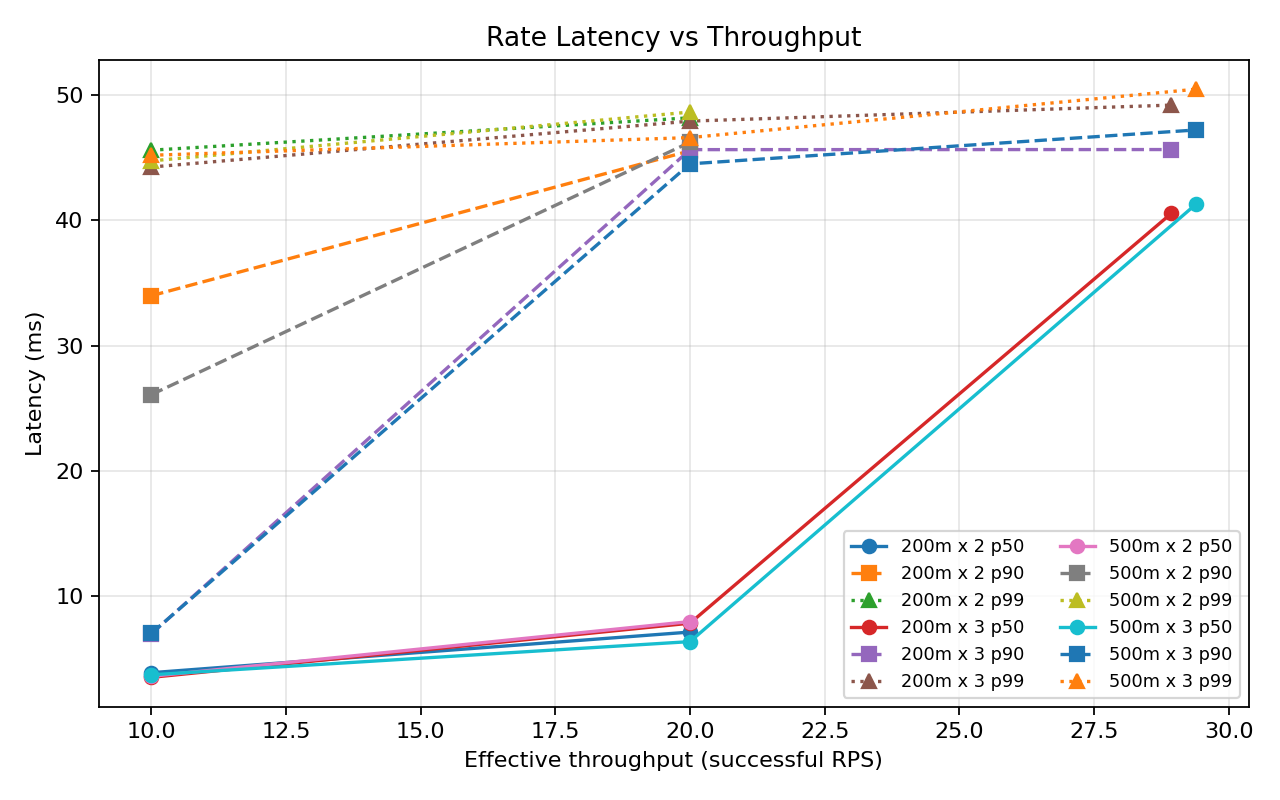
\includegraphics[width=\columnwidth]{report_figures/latency_vs_throughput.png}
\caption{Latency-throughput behavior for \texttt{rate}.}
\label{fig:rate-latency}
\end{figure}

The focused results sharpen our understanding of the bottleneck in three ways.

First, the 200m configurations show clear CPU throttling. At 200m with two replicas, one pod accumulated 252{,}873 throttled microseconds and another still saw 16{,}074. At 200m with three replicas, throttling rose to 422{,}359 and 49{,}029 microseconds on two pods. These runs therefore fail under a genuine CPU-control constraint.

Second, the 500m configurations still scale poorly even after throttling disappears. For both 500m with two replicas and 500m with three replicas, the detailed report shows zero throttled microseconds, yet the measured MSC remains only 10 and 20 RPS in the focused cold-cache study. This means the service does not recover simply by removing the CPU cap.

Third, the failure mode at 500m points away from a memory bottleneck and toward a cold-cache coordination problem. The diagnosis report explicitly notes low memory pressure, and the average observed pod CPU remains around 10m even when success-rate violations appear. That combination is important: the service is not failing because it fully consumes CPU or memory. It is failing while spending substantial time waiting on backend work, request fan-out, cache-miss handling, serialization, or network coordination. This interpretation is also consistent with the measured run-queue wait times being very small while the service still fails to scale linearly.

Taken together, these observations make our explanation more precise than simply saying that \texttt{rate} is ``slow.'' At low CPU budgets, Linux cgroup throttling is a direct limiter. At higher CPU budgets, the bottleneck shifts to the cold-cache execution path and the service's coordination overhead per request. In practical terms, adding replicas alone is not enough; improving cache-hit behavior, reducing downstream work per request, or restructuring request processing is more likely to help.

This also helps explain the live-versus-sandbox \texttt{search} gap. Because live \texttt{search} must wait on real \texttt{rate} responses, the weak scaling and latency sensitivity of \texttt{rate} are inherited by the live \texttt{search} path. Once we replace \texttt{rate} with deterministic replay, that inherited bottleneck is removed, and the measured throughput moves much closer to the intrinsic behavior of \texttt{search}.

\section{Discussion}
Three main conclusions emerged from the repository and our experiments.

First, sandboxing is most valuable for dependency-heavy services. The \texttt{search} pipeline shows that capture-and-replay can preserve realistic semantics while making experiments more reproducible and much easier to reason about than full end-to-end reruns.

Second, MSC is highly service-specific. Within the same application and under the same SLO, some services scale well with more resources, while others do not. This validates the need for per-service capacity planning rather than a single autoscaling rule for the entire application.

Third, raw resource provisioning is not the same as real scaling. Our results repeatedly show that adding CPU or replicas can help only when the service architecture is ready to use them. Where the runtime is dominated by cache misses, synchronization, or request amplification, additional resources have diminishing returns.

A fourth conclusion follows from the live-versus-sandbox comparison. End-to-end measurement alone can be misleading when the goal is per-service capacity analysis. Live \texttt{search} looked severely constrained across almost all configurations, but the sandboxed results showed that \texttt{search} itself was not the main limiter. In other words, the experiment design determines what question the result answers. The live runs answer ``how does the whole dependency chain behave when \texttt{search} is resized?'' The sandboxed runs answer ``what is the capacity of \texttt{search} itself under realistic request semantics?'' For this project, we needed both questions, but only sandboxing let us answer the second one correctly.

From a systems perspective, this separation is useful for tuning decisions. If the live result is poor but the sandboxed result is strong, then optimization effort should focus on the dependencies or their interaction patterns. If both results are poor, then the service under test is likely a primary bottleneck. Our data places \texttt{search} in the first category and \texttt{rate} in the second.

Our current implementation also has limitations. The dependency sandbox is specialized to the \texttt{search} path rather than generalized to every non-leaf service. The experiments are Minikube-first, so the exact numeric results are cluster-specific. Finally, the best \texttt{search} run is right-censored at 500 RPS because that was the configured maximum test rate.

\section{Threats to Validity and Future Work}
There are several important caveats to our current results. First, the experiments were run on a Minikube-centered environment, so absolute MSC values may shift on larger multi-node clusters or under different network conditions. Second, the live-versus-sandbox comparison depends on the captured traffic corpus. Although the corpus is derived from real application requests, it still represents only a finite slice of the possible workload space. Third, the \texttt{search} results at 500m CPU are censored at the configured maximum of 500 RPS, so the best sandboxed configurations may have additional headroom.

Future work can extend the system in three directions. One direction is breadth: sandbox additional non-leaf services if their downstream fan-out becomes important to study. A second direction is depth: add richer prediction models that incorporate memory, observed CPU, or non-linear interaction terms. A third direction is automation: use the measured MSC data to recommend deployment configurations or to guide autoscaling policies more directly. Even in its current form, however, the workflow already demonstrates that service-level sandboxing and lightweight predictive modeling can work together effectively.

\section{Conclusion}
We developed a practical sandbox-based capacity-analysis framework for the DeathStarBench Hotel Reservation application. The framework captures real gRPC traffic, normalizes it into replay fixtures, deploys a Kubernetes sandbox for \texttt{search}, measures MSC through binary-search load testing, and complements the main sweeps with both predictive modeling and targeted bottleneck diagnosis.

Our results show four clear outcomes. \texttt{search} scales strongly when its downstream dependencies are sandboxed through deterministic replay. Live \texttt{search}, by contrast, remains strongly P90-latency-bound, which confirms that sandboxing is necessary if we want to measure the capacity of \texttt{search} itself rather than the capacity of the whole dependency chain. \texttt{reservation} scales well with added CPU and replicas. \texttt{rate} is the dominant bottleneck candidate because of throttling at low CPU limits and cold-cache coordination overhead at higher limits. The added prediction model further shows that simple per-service linear fitting can already provide useful MSC estimates for unseen CPU settings, achieving 16.4\% MAPE on the 150m validation runs.

Overall, we found that sandbox-based microservice analysis provides much deeper operational insight than conventional end-to-end benchmarking alone. It lets us separate dependency effects from service effects, reason about replica scaling more accurately, and move from raw measurements toward practical capacity prediction.

\begin{thebibliography}{1}

\bibitem{jindal2019}
A.~Jindal, V.~Podolskiy, and M.~Gerndt, ``Performance modeling for cloud microservice applications,'' in \emph{Proc. ACM/SPEC Int. Conf. on Performance Engineering (ICPE)}, 2019.

\bibitem{gan2019}
Y.~Gan et al., ``An open-source benchmark suite for microservices and their hardware-software implications for cloud and edge systems,'' in \emph{Proc. ASPLOS}, 2019.

\end{thebibliography}

\end{document}
